%\documentclass[border={5pt, 15pt, 10pt, 5pt}, convert={density=400}]{standalone}
\documentclass[border={5pt, 15pt, 10pt, 5pt}, convert={density=140}]{standalone}

%\usepackage[T1]{fontenc}
%\usepackage[default]{raleway}
%\usefonttheme[onlymath]{serif}% raleway looks ugly in math; this uses standard serif math font

\renewcommand{\familydefault}{\sfdefault}

\usepackage{tikz, xcolor}
\usetikzlibrary{shapes.geometric, backgrounds, positioning, decorations.markings} 
\usetikzlibrary{arrows.meta, graphs, shapes.misc} 
\usetikzlibrary{calc}

\definecolor{vq_background}{RGB}{8,31,77}
\definecolor{vq_background2}{RGB}{12,47,116}
\definecolor{vq_background3}{rgb}{0.149,0.388,0.6}
\definecolor{vq_green}{RGB}{0,235,210}
\definecolor{vq_green_light}{RGB}{204,251,246}% green with 80% white added
\definecolor{vq_blue}{RGB}{0,173,234}

%\pagecolor{white}

\begin{document}



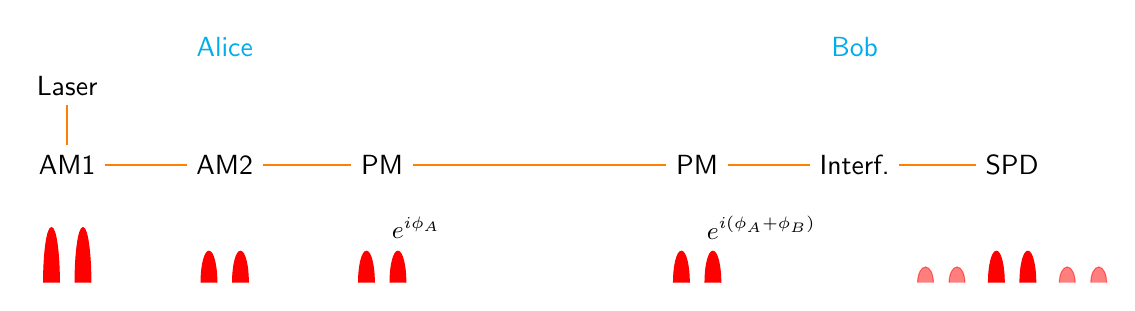
\begin{tikzpicture}
    \node (l) at (0,1) {Laser};
    \node (am) at (0,0) {AM1};
    \node (am2) at (2,0) {AM2};
    \node (pm1) at (4,0) {PM};
    \node (pm2) at (8,0) {PM};
    \node (i) at (10,0) {Interf.};
    \node (spd) at (12,0) {SPD};
    \draw[orange, thick] (l) -- (am) -- (am2) -- (pm1) -- (pm2) -- (i) -- (spd);
    \node[text=vq_blue] (Alice) at (2,1.5) {Alice};
    \node[text=vq_blue] (Alice) at (10,1.5) {Bob};

    \draw[red, fill] (-0.1,-1.5) arc (0:180:0.1 and 0.7);
    \draw[red, fill] (0.1,-1.5) arc (180:0:0.1 and 0.7);
    
    \draw[red, fill] (1.9,-1.5) arc (0:180:0.1 and 0.4);
    \draw[red, fill] (2.1,-1.5) arc (180:0:0.1 and 0.4);

    \draw[red, fill] (3.9,-1.5) arc (0:180:0.1 and 0.4);
    \draw[red, fill] (4.1,-1.5) arc (180:0:0.1 and 0.4);
    \node[anchor=west, font=\small] at (4.0, -0.8) {$e^{i\phi_A}$};

    \draw[red, fill] (7.9,-1.5) arc (0:180:0.1 and 0.4);
    \draw[red, fill] (8.1,-1.5) arc (180:0:0.1 and 0.4);
    \node[anchor=west, font=\small] at (8.0, -0.8) {$e^{i(\phi_A + \phi_B)}$};
    
    \draw[red, fill] (11.9,-1.5) arc (0:180:0.1 and 0.4);
    \draw[red, fill] (12.1,-1.5) arc (180:0:0.1 and 0.4);
    \draw[red, fill, opacity=0.5] (11.0,-1.5) arc (0:180:0.1 and 0.2);
    \draw[red, fill, opacity=0.5] (11.2,-1.5) arc (180:0:0.1 and 0.2);
    \draw[red, fill, opacity=0.5] (12.8,-1.5) arc (0:180:0.1 and 0.2);
    \draw[red, fill, opacity=0.5] (13.0,-1.5) arc (180:0:0.1 and 0.2);

\end{tikzpicture}


\end{document}











